\appendix
\section{Alternative iFlow model}
A comment in the files mentioned an error in the implementation because the Softplus function was applied to $\xi$ as well as $\eta$ from the natural parameters $\mathbf{\lambda (u)}$. An alternative version of the implementation was also tested where the Softplus activation function was only exerted on $\xi$, as there are no constraints on the sign of $\eta$. 

% MCC of 0.72 (0.057)
The results obtained using this method were approximately the same as the original performance of the iFlow. A mean MCC of 0.72 with a standard deviation of 0.057 was achieved. Because these results were not a significant improvement, it was decided to include this experiment as an appendix.  

\section{Baseline improvement experiments}

The table below shows the results of experiments with changing the iVAE architecture to increase complexity. As shown, adding skip connections or layer normalisation to the architecture did not increase performance with respect to the unchanged baseline. Due to the high training time, no additional experiments could be done.

\label{sec:baselineexperiments}
\begin{center}
\begin{tabular}{ccccc} 
     \toprule
     addition & NUM\_HIDDEN & NUM\_LAYERS & AVG MCC \\
     \midrule
     - & 50 & 3 & 0.483 (\textpm 0.059)\\
     residual connections & 50 & 3 & 0.474 (\textpm 0.053)\\
     layer normalisation & 50 & 3 & 0.461 (\textpm 0.051)\\
     \bottomrule\\
\end{tabular}
\end{center}

\newpage
\section{Visualizations for Fixed iVAE}
\label{sec:appendixC}

\begin{figure}[ht]
    \centering
    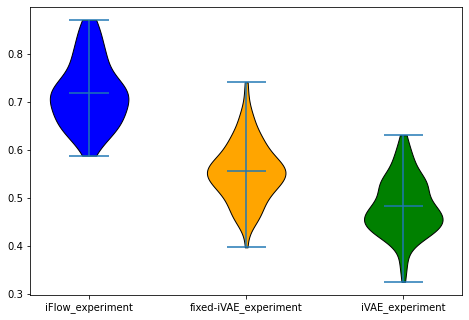
\includegraphics[width=0.5\textwidth]{scores/violin_plot_fixed.png} 
    \caption{Alternative visualisation of the MCC scores obtained by the models, including the fixed iVAE.} 
    \label{fig:violinplot} 
\end{figure}

\begin{figure}[ht]
    \centering
    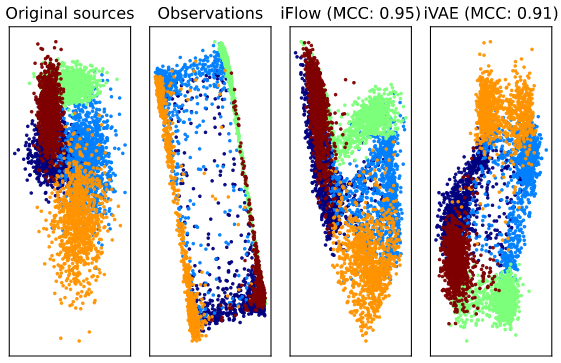
\includegraphics[width=0.5\textwidth]{Reproducibility_Challenge_2020/IMG/2D_perf/2D_performance_fixed_iVAE.png} 
    \caption{Visualisation of 2D-cases, comparing iFlow to the fixed version of iVAE.} 
    \label{fig:fixedMCCscores} 
\end{figure}

\begin{figure}[!htbp]
    \centering
    \begin{minipage}[b]{\textwidth}
        \centering
       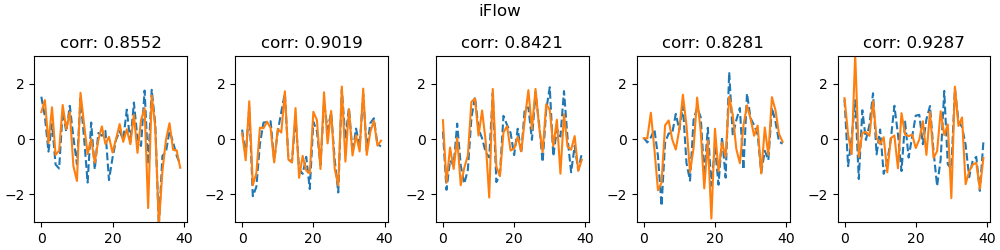
\includegraphics[width=0.8\textwidth]{latent_corr/best_iFlow_42.png}
    \end{minipage}
    \begin{minipage}[b]{\textwidth}
    \centering
       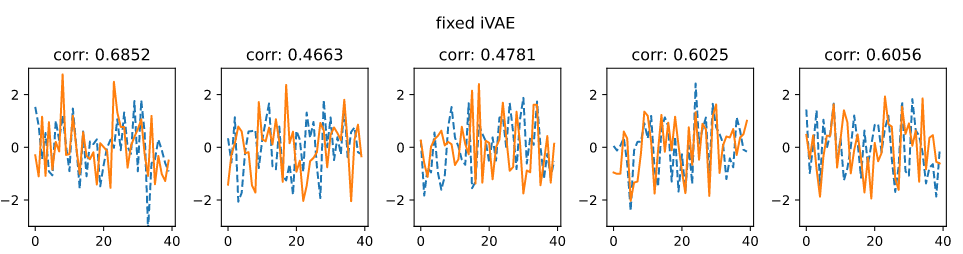
\includegraphics[width=0.8\textwidth]{IMG/latent_corr/fixed_iVAE_42.png}
    \end{minipage}
    \caption{Comparison of the latent variables recovered by the models (orange lines) to the true latent variables (dashed blue lines) for individual dimensions. This figure shows results for the seed that resulted in the best iFlow performance.}
    \label{fig:latentcorr_fixed1}
\end{figure}

\begin{figure}[!htbp]
    \centering
    \begin{minipage}[b]{\textwidth}
        \centering
       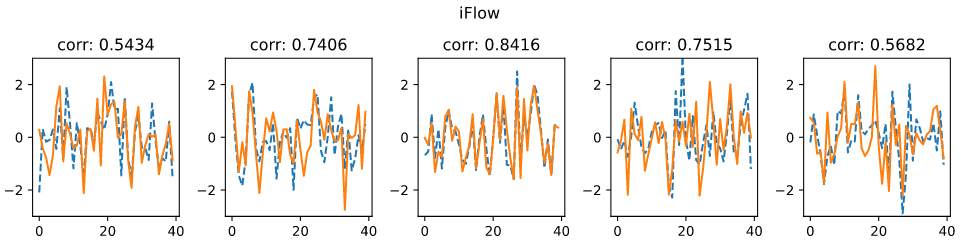
\includegraphics[width=0.8\textwidth]{Reproducibility_Challenge_2020/IMG/latent_corr/iFlow_X.png}
    \end{minipage}
    \begin{minipage}[b]{\textwidth}
    \centering
       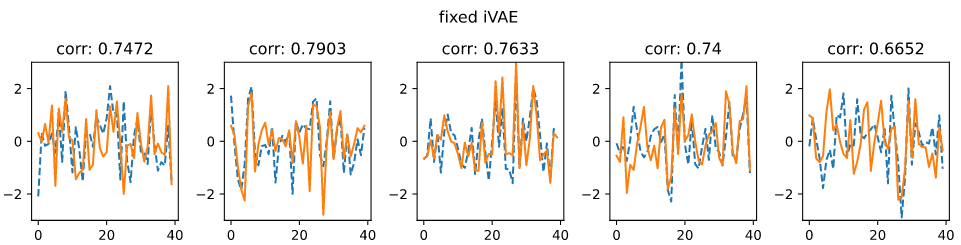
\includegraphics[width=0.8\textwidth]{Reproducibility_Challenge_2020/IMG/latent_corr/best_fixed_iVAE_X.png}
    \end{minipage}
    \caption{Comparison of the latent variables recovered by the models (orange lines) to the true latent variables (dashed blue lines) for individual dimensions. This figure shows results for the seed that resulted in the best fixed iVAE performance.}
    \label{fig:latentcorr_fixed1}
\end{figure}
